\documentclass[12pt]{article}

\usepackage[T1]{fontenc}
\usepackage[utf8]{inputenc} % L'encodage du document
\usepackage[french]{babel} % Des options supplémentaires pour que le document soit en français (noms de sections, etc.)
\usepackage{geometry}
\geometry{hscale=0.80,vscale=0.80,centering} % Permet de définir les marges (ici 10% de chaque côté)
\usepackage{amsmath}
\usepackage{amssymb}
\usepackage{amsthm} % For theorem-like environments
\usepackage{graphicx} % Ajout du package graphicx
\usepackage{minted}
\usepackage{fixltx2e}
\usepackage{array}
\usepackage{lettrine}
\usepackage{tikz}
\usetikzlibrary{angles,quotes}

\newcolumntype{C}[1]{>{\centering\arraybackslash}m{#1}}
\newcolumntype{L}[1]{>{\raggedright\arraybackslash}m{#1}}
\newcolumntype{N}{@{}m{0pt}@{}}

\newcounter{definitioncounter}
\renewcommand{\thedefinitioncounter}{\arabic{definitioncounter}}

\newcommand{\definition}[1]{%
    \par\noindent\textbf{Définition \refstepcounter{definitioncounter}\thedefinitioncounter.} #1 \vspace{0.5\baselineskip}
}

\newcommand{\fig}[1]{
    F\resizebox{!}{1.3ex}{IGURE} #1
}

\newcounter{propositioncounter}
\renewcommand{\thepropositioncounter}{\arabic{propositioncounter}}

\newcommand{\proposition}[1]{%
    \par\noindent\textbf{Proposition \refstepcounter{propositioncounter}\thepropositioncounter.} #1 \vspace{0.5\baselineskip}
}

\setlength{\parindent}{15pt} % Fixe l'indentation en début de paragraphe
\setlength{\parskip}{10pt} % Fixe l'espacement entre paragraphes

\begin{document}
\title{Simuler les feux de forêt}
\date{\today}
\author{Victor Sarrazin}

\maketitle

\section*{Introduction}

Avec le changement climatique, les feux de forêt sont de plus en plus fréquents et dévastateurs, à l'image de ceux en Californie en janvier 2025.

Dans ce cadre, les modélisations informatiques des feux de forêt permettent de simuler l'évolution des feux, afin de prévoir les zones à risques. Mais les simulations informatiques permettent aussi de tester l'impact de certaines transformations sur ces feux, afin de trouver des manières de réduire l'impact des catastrophes, sans pour autant dénaturer les forêts.

\section{Automates cellulaires}

\subsection{Généralités}

Pour réaliser nos modélisations, nous allons utiliser des automates cellulaires. Les automates cellulaires permettent de représenter des systèmes avec des intéractions locales entre les éléments qui constituent ces derniers. Les automates cellulaires ont notamment été popularisés avec \textit{Le~Jeu~de~la~Vie} de \textit{Conway}.

\definition{Un automate cellulaire est la donnée d'un triplet $(Q, M, f)$ avec :\begin{itemize}
    \item $Q$ un ensemble d'états
    \item $M$ une matrice de taille $n \times m$, où chaque $m_{i,j}$ représente une case de la grille
    \item $f : \mathcal{M}_{n,m}(Q) \longrightarrow \mathcal{M}_{n,m}(Q)$ une \textit{fonction de transition} qui à une grille renvoie la grille suivante
\end{itemize}}

La définition de la fonction de transition dépend donc du type de voisinage utilisé. Il existe deux principaux types de voisinages, celui de \textit{von Neumann} et celui de \textit{Moore}. Nous avons choisi d'utiliser le voisinage de \textit{Moore} pour nos modélisations pour prendre en compte le plus d'intéractions possibles, celui de \textit{von Neumann} étant limitant notamment sur les diagonales.

\definition{Le voisinage de \textit{Moore} est composé du noeud et de ses 8 voisins.}

\begin{figure}[!h]
    \centering
    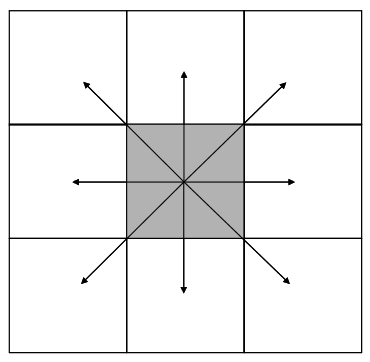
\includegraphics[width=0.20\linewidth]{pictures/moore.png}
    \caption{Voisinage de Moore}
    \label{fig:enter-label}
\end{figure}

Il serait possible dans une optique d'avoir des modèles encore plus précis d'utiliser des voisinages de \textit{Moore} étendus, avec plusieurs rayons de voisins, mais dans un soucis de simplicité nous nous sommes restreints à un rayon.

\subsection{Représentation d'un forêt}

Afin de représenter une forêt avec un automate cellulaire nous avons défini une liste d'état que les cases pouvaient prendre.

\definition{Les états possibles sont :
\begin{itemize}
    \item Arbres
    \item Arbres denses
    \item Champs
    \item Feu
    \item Case brulée\textsuperscript{*}
    \item Eau\textsuperscript{*}
\end{itemize}
A noter que les cases $(*)$ ne peuvent brûler.}

Nous avons choisi de travailler avec une matrice de taille $256 \times 256$ pour des raisons techniques : au delà le temps de calcul devenait trop long et l'ajout de lignes/colonnes ne représentait pas un intérêt suffisant pour le faire par rapport au temps de calcul que celà impliquait.

\section{Modèle d'Alexandridis}

Dans un premier temps il est possible de faire une modélisation naïve des feux de forêt en associant à chaque case une probabilité fixe de brûler si un de ses voisins est en feu. Une telle tentative a été réalisée avec des résultats quelque peu satisfaisants, c'est pourquoi l'objectif de cette deuxième partie est de voir un modèle plus poussé de modélisation des feux de forêts, dit modèle d'\textit{Alexandridis}.

\subsection{Présentation du modèle}

Le modèle d'\textit{Alexandridis} prend en compte divers phénomènes pour modéliser cette propagation. Dans la suite nous avons choisi de nous restreindre à la densité de végétation, au type de végétation ainsi qu'au vent dans la zone. Le modèle original quant à lui prend aussi en compte l'élévation du terrain.

\proposition{On utilise les règles de transition suivantes, pour $(i,j) \in \mathbb{N}^2$, $t \in \mathbb{N}$ :
\begin{itemize}
    \item Si $m_{i,j} (t) = $ \mintinline{latex}{feu} alors $m_{i,j} (t+1) = $ \mintinline{latex}{brulé}
    \item Si $m_{i,j} (t) = $ \mintinline{latex}{feu} alors $m_{i \pm 1,j \pm 1} (t+1) = $ \mintinline{latex}{feu} avec une probabilité $p_b$
    \item Si $m_{i,j} (t) = $ \mintinline{latex}{brulé} alors $m_{i,j} (t+1) = $ \mintinline{latex}{brulé}
\end{itemize}}

\proposition{La probabilité $p_b$ qu'une case brûle est définie par
$p_b = p_h (1 + p_{veg}) (1 + p_{den}) p_{vent}$ avec $p_h = 0.27$ une constante, $p_{veg}$ et $p_{den}$ relatives au type de case.
}

\begin{figure}[!h]
    \centering
    \renewcommand{\arraystretch}{2}
    \setlength{\extrarowheight}{-3pt}
    \begin{tabular}{ |>{\centering\arraybackslash}p{4cm}|>{\centering\arraybackslash}p{2cm}|>{\centering\arraybackslash}p{2cm}| }
        \cline{2-3}
        \multicolumn{1}{c|}{} & $p_{veg}$ & $p_{den}$ \\
        \hline 
        Arbres & $0.3$ & $0.3$ \\ 
        \hline
        Arbres denses & $0.3$ & $0$ \\ 
        \hline
        Champs & $-0.1$ & $0$ \\
        \hline 
    \end{tabular}
    \caption{Probabilités $p_{veg}$ et $p_{den}$ selon le type de végétation}
\end{figure}

\proposition{La probabilité $p_{vent}$ liée au vent est définie par
\\ $p_{vent} = \exp (0.045 v) \times \exp (0.131 v \times (\cos (\theta) - 1))$ avec $\theta$ l'angle entre la propagation du feu et la direction du vent, et $v$ la vitesse du vent (en $m/s$)
}

\begin{figure}[!h]
    \centering
    \begin{tikzpicture}[> = stealth]
        \coordinate (a) at (1,4);
        \coordinate (b) at (2,5);
        \coordinate (c) at (5,4);
        \coordinate (d) at (6,4);
        \coordinate (e) at (9,5);
        \coordinate (f) at (10,4);
        
        \draw pic[draw,fill=green!30,angle radius=1cm,"$\theta_1$" shift={(6mm,1mm)}] {angle=c--a--b};
        \draw pic[draw,fill=green!30,angle radius=2cm,"$\theta_2$" shift={(6mm,1mm)}] {angle=f--d--e};
        
        \draw[ultra thick,red, ->]  (a) -- node[above left] {\normalsize Vent} (b);
        \draw[ultra thick,blue,->]  (a) -- node[below] {\normalsize Propagation du feu} (c);

        \draw[ultra thick,red, ->]  (d) -- node[above left] {\normalsize Vent} (e);
        \draw[ultra thick,blue,->]  (d) -- node[below] {\normalsize Propagation du feu} (f);
    \end{tikzpicture}
    \caption{Schémas pour le vent}
\end{figure}
\subsection{Résultats}

Dans un premier temps comparons les résultats de la modélisation naïve et celui du modèle d'\textit{Alexandridis} :

\begin{figure}[!h]
    \centering
    \begin{minipage}{0.35\textwidth}
      \centering
      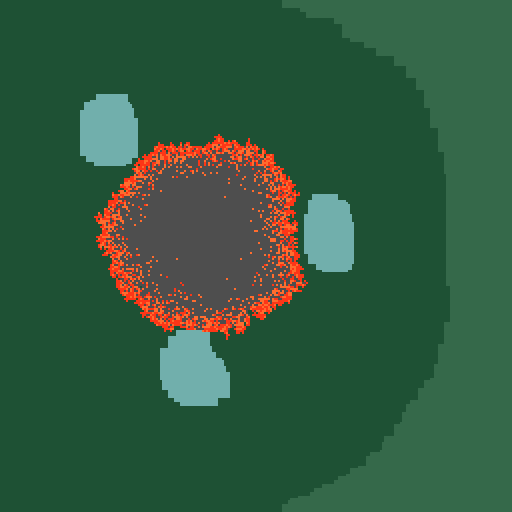
\includegraphics[width=.8\linewidth]{pictures/model1/land_200.png}
      \caption{Solution naïve}\label{Fig:Data1}
    \end{minipage}
    \hfil
    \begin{minipage}{0.35\textwidth}
      \centering
      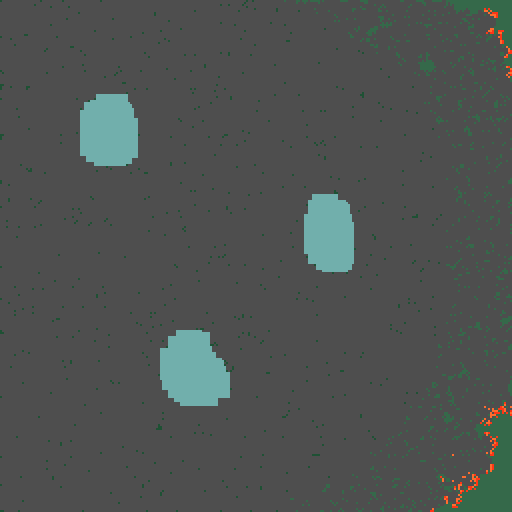
\includegraphics[width=.8\linewidth]{pictures/model2/land_200_nowind.png}
      \caption{\textit{Alexandridis}}\label{Fig:Data2}
    \end{minipage}
 \end{figure}

On remarque que la solution naïve a une propagation plus lente et un front de feu plus étendu que celui du modèle d'\textit{Alexandridis}.

Comparons maintenant deux modélisations avec des densités de végétation différentes, et sous $15 m/s$ de vent vers l'est :

\begin{figure}[!h]
    \centering
    \begin{minipage}{0.35\textwidth}
      \centering
      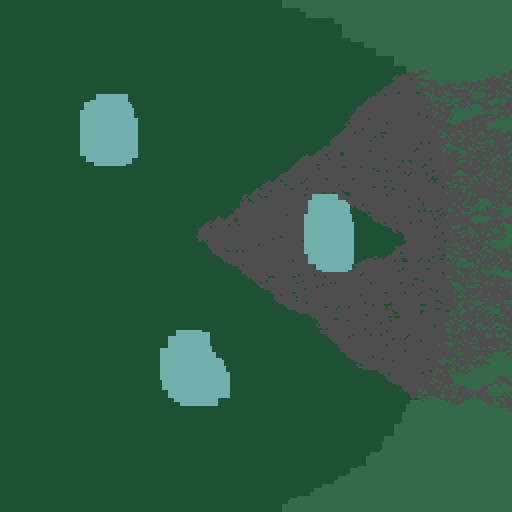
\includegraphics[width=.8\linewidth]{pictures/model2/land_200_wind_notdense.png}
      \caption{Végétation normale}\label{Fig:Data3}
    \end{minipage}\hfil
    \begin{minipage}{0.35\textwidth}
      \centering
      
\includegraphics[width=.8\linewidth]{pictures/model2/land_200_wind_dense.png}
      \caption{Végétation dense}\label{Fig:Data4}
    \end{minipage}
 \end{figure}

On remarque principalement deux effets notoires sur les deux modélisations.

D'une part, la progression dans une végétation normale est moins rapide (ce qui fait sens empiriquement), et donc le front est moins étendu. La surface brulée dans le cas de la densité normale présente aussi des trous là où celle de la densité élevée est lisse, ce phénomène est expliqué par le fait que $p_b$ est plus élevée pour une densité plus forte.

D'autre part, dans les deux modélisations on voit clairement l'impact du vent : le front de feu s'est déplacé suivant un cône poussé par le vent.

\subsection{Considérations algorithmiques}

Cette sous partie a pour objectif de rendre compte de l'implémentation de la modélisation réalisée et de comprendre le choix de $256 \times 256$.

Voici les complexités des différentes fonctions créés :

\begin{itemize}
    \item Calcul de $p_b$ : $O(1)$
    \item Calcul du passage de $t$ à $t+1$ : $O(n^2)$ avec $n$ la longueur de la grille, avec une estimation de $100$ opérations élémentaires pour chaque case
    \item Affichage de l'état $t$ : $O(m^2 \times n^2)$ avec $n$ la longueur de la grille et $m$ la taille d'une case représentée sur l'écran
\end{itemize}

Ainsi pour $N$ itérations, on trouve une complexité totale de $O(m^2 \times n^2 \times N)$, numériquement avec $n$ = 256, $m$ = 2 et $N$ = 200 on trouve $\approx 10^5$, et donc on en déduit grossièrement $\approx 10^7$ opérations élémentaires, pour un temps de calcul d'environ $5$ secondes.

On comprend donc pourquoi augmenter la valeur de $n$ (toutes choses égales par ailleurs) ou de $N$ conduirait à des simulations plus longues.

\section{Transformations}

Puisque nous avons maintenant un modèle pour réaliser des simulations, nous allons nous intéresser aux transformations réalisables, notamment ici dans le cadre de cette étude aux tranchées et chemins.

\subsection{Explications}

Nous allons donc considérer la transformation suivante : l'ajout de tranchées ou de chemins forestiers, des transformations légères dans les forêts qui permettent de ne pas dénaturer ces dernières.

\proposition{On ajoute un nouvel état Chemins/Tranchées avec $p_{veg} = -0.55$ et $p_{den} = 0$ à notre modèle.}

\subsection{Résultats}

L'objectif est maintenant de voir l'impact des tranchées, avec des configurations différentes de vent et de longueur de tranchées.

\subsubsection{Tranchées/Sans tranchées}

La première comparaison intéressante et de regarder la différence de propagation de feu avec et sans tranchées.

\begin{figure}[!h]
    \centering
    \begin{minipage}{0.35\textwidth}
      \centering
      
\includegraphics[width=.8\linewidth]{pictures/trans/no_treach.png}
      \caption{Sans tranchées}\label{Fig:Data5}
    \end{minipage}\hfill
    \begin{minipage}{0.35\textwidth}
      \centering
      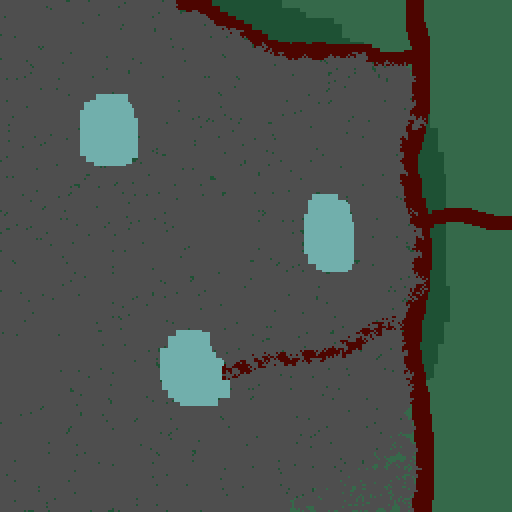
\includegraphics[width=.8\linewidth]{pictures/trans/treach.png}
      \caption{Avec tranchées}\label{Fig:Data6}
    \end{minipage}
\end{figure}

On constate donc en comparant la\fig{8}et la\fig{9}que la présence de tranchées permet de bloquer le feu. Il est possible de critiquer le résultat dans la mesure où on a un nombre d'itérations limitées (ici $200$), et que le feu aurait donc plus de temps pour se propager.

\subsubsection{Vent faible/Vent fort}

Dans un deuxième temps, comparons deux situations de vent différentes, dans le même sens mais avec une vitesse différente.

\begin{figure}[!h]
    \centering
    \begin{minipage}{0.35\textwidth}
      \centering
      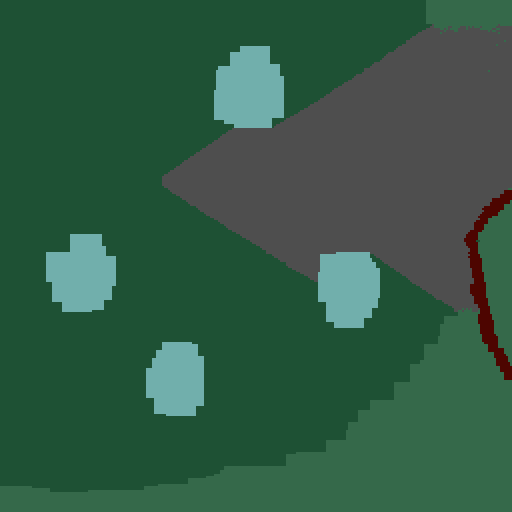
\includegraphics[width=.8\linewidth]{pictures/trans/treach_15.png}
      \caption{$15$ m/s de vent}\label{Fig:Data7}
    \end{minipage}\hfill
    \begin{minipage}{0.35\textwidth}
      \centering
      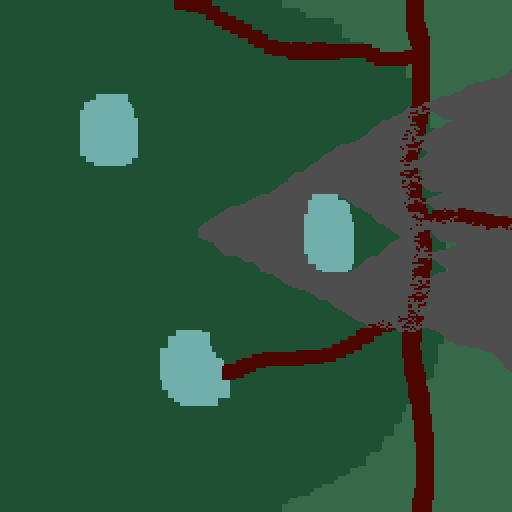
\includegraphics[width=.8\linewidth]{pictures/trans/treach_30.png}
      \caption{$30$ m/s de vent}\label{Fig:Data8}
    \end{minipage}
\end{figure}

On constate donc en comparant la\fig{10}et la\fig{11}que la situation où le vent est plus fort rend moins efficace la tranchée/le chemin. Ce résultat est assez logique empiriquement dans la mesure où un vent plus fort permet au feu d'aller plus loin, et donc de passer plus facilement la tranchée.

Il est tout de même intéressant de mentionner que même si le feu passe outre la tranchée, moins de 25\% de cette dernière est brulée à la fin (dans la zone impactée par le feu)

\subsubsection{Tranchée mince/Tranchée large}

Dans un dernier temps, comparons deux tailles de tranchée.

\begin{figure}[!h]
    \centering
    \begin{minipage}{0.35\textwidth}
      \centering
      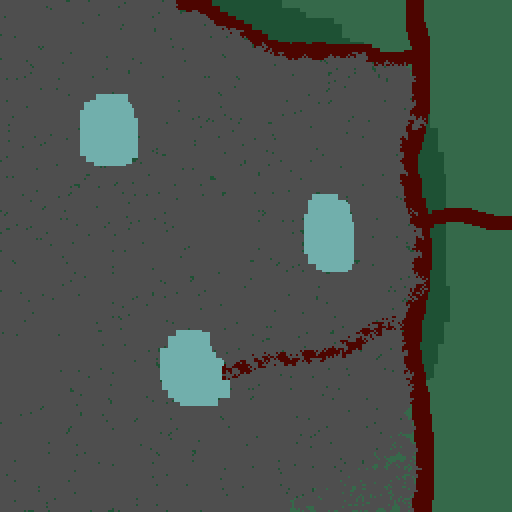
\includegraphics[width=.8\linewidth]{pictures/trans/treach.png}
      \caption{Tranchée de $8$m}\label{Fig:Data9}
    \end{minipage}\hfill
    \begin{minipage}{0.35\textwidth}
      \centering
      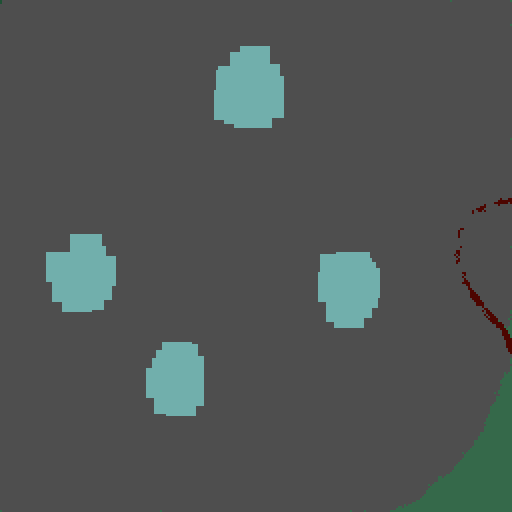
\includegraphics[width=.8\linewidth]{pictures/trans/little_treach.png}
      \caption{Tranchée de $4$m}\label{Fig:Data10}
    \end{minipage}
\end{figure}

On constate en comparant la\fig{12}et la\fig{13}que plus une tranchée est large, plus elle réduit les possibilités de propagation du feu. Entre ces deux simulations c'est la grande tranchée verticale qui a été réduite horizontalement et on voit bien l'impact de ce changement.

De plus on observe sur la\fig{13}que le front de feu est encore présent, et donc que si la simulation durait plus longtemps une zone encore plus vaste serait brûlée.

\subsection{Possibles améliorations}

Il est possible d'aller plus loin dans les simulations, nous nous sommes limités à un modèle intermédiaire, prenant en compte le type de végétation, la densité de cette dernière ainsi que le vent.

Il serait donc envisageable de prendre en compte d'autres paramètres dans la modélisation tels que l'élévation, l'humidité ou la température.

De plus il est aussi possible de considérer d'autres transformations telles que la réduction de la densité de végétation car on a vu en\fig{7}qu'une végétation dense favorisait la propagation, ou encore considérer une intéraction plus complexe avec les cours d'eau/lacs, ici considérés uniquement comme des zones bloquant totalement le feu alors qu'elles peuvent lui permettre de tout de même progresser.

\section{Annexe}

\subsection{Choix d'implémentation}

Pour implémenter les différents modèles nous avons choisi d'utiliser le langage \mintinline{latex}{C99}. Le choix du langage a été motivé principalement par deux aspects :

\begin{itemize}
    \item Le \mintinline{latex}{C} permet par son bas niveau de gagner un certain temps d'exécution par rapport à d'autres langages, utile ici au vu du nombre de calculs à effectuer dans nos grilles.
    \item Le \mintinline{latex}{C} étant plus utilisé que le \mintinline{latex}{OCaml}, il bénéficie par conséquent de plus de bibliothèques externes.
\end{itemize}

Nous avons utilisé les bibliothèques non standard suivantes :

\begin{itemize}
    \item \mintinline{latex}{SDL2} : Pour réaliser une interface graphique afin de visualiser les évolutions.
    \item \mintinline{latex}{cJSON} : Pour manipuler des fichiers \mintinline{latex}{JSON} et représenter les grilles afin de pouvoir les importer.
    \item \mintinline{latex}{png} : Pour créer des fichiers \mintinline{latex}{PNG} et les manipuler en \mintinline{latex}{C} afin d'exporter nos simulations.
\end{itemize}

Pour créer plus facilement les grilles, nous avons créé un site web avec \mintinline{latex}|React.JS|.

\end{document}